\documentclass[9pt]{beamer}
\renewcommand\textbullet{\ensuremath{\bullet}}

\usepackage{sty/opencg3-spec}
\usepackage{sty/opencg3-spec-beamer}
\usepackage{xspace,bookmark,lmodern,mathtools,color,multido,ulem,upquote,tabularx,hhline,multirow}
\usepackage[T1]{fontenc}
\usefonttheme[onlymath]{serif}
\setcounter{tocdepth}{4}

\newcommand{\Version}[0]{Version 0.3.5}
\newcommand{\PrjName}{OpenCG\texorpdfstring{\textsuperscript{3}}}
\newcommand{\PrjNameFull}{\LARGE Open Command-oriented\\Geometric Graphics Generator}
\newcommand{\PrjSpec}{\PrjName{} Specification \Version}

\title[\PrjSpec]{\PrjNameFull}
\subtitle{\small \PrjSpec}


\author[KVD \and ADL]{Dong Nai-Jia \inst{1} \and Lin Yong-Hsiang \inst{2}}
\institute{\inst{1} National Chiao Tung University\\Department of Computer Science \and
           \inst{2} National Taiwan University\\Department of Agricultural Chemistry}
\date[\today]{\today}


\begin{document}
\beamertemplatenavigationsymbolsempty

\section{OpenGC3}

\begin{frame}
	\titlepage
\end{frame}


\section{Overview}

\subsection{Language}

\subsubsection{Token}

\begin{frame}[t] \frametitle{Command Tokens}

	\begin{block}{Regular Expressions}
		$\MSN \coloneqq \{\ \alpha \mid \alpha \in \texttt{[0-9]+} \ \}$ \\ [.24em]
		$\MSR \coloneqq \{\ \alpha \mid \alpha \in \texttt{[+\textbackslash-]?([0-9]*[.])?[0-9]+}\ \}$ \hfill
		$\Rightarrow \MSR \supset \MSN \ $ \\ [.24em]
		$\MSS \coloneqq \{\ \alpha \mid \alpha \in \texttt{\Quote(.*?)\Quote|[.0-9A-Za-z+\textbackslash-]+} \ \}$ \hfill
		$\Rightarrow \MSS \supset \MSR \ $ \\ [.24em]
		$\MSW \coloneqq \{\ \alpha \mid \alpha \in \texttt{[ \textbackslash{}t]} \}$ \hfill whitespace
	\end{block}

	\begin{block}{Descriptions}
		\begin{itemize}
			\item The matching mechanism abides by the maximal munch rule.
			\item Each command is whitespace-insensitive except being quoted by a pair of single quotation marks (\Quote).
		\end{itemize}
	\end{block}

\end{frame}

\subsubsection{Grammar}

\begin{frame}[t] \frametitle{Command Grammars}

	\begin{block}{Context-Free Expansions}
		$\left.\CMD \EXP \ARG \CMD \SEP \,\text{;}\, \SEP \,\texttt{EOL} \right.$ \\ [.24em]
		$\left.\ARG \EXP \TUP(\ARG) \SEP \VCT(\ARG) \SEP \SET(\ARG) \SEP
		 \LST(\ARG) \SEP \LST(\ARG, \ARG, \cdots, \ARG) \SEP \MSN \SEP \MSR \SEP \MSS \right.$ \\ [.27em]
		$\left.\text{%
		\begin{tabular}{@{}l}%
			$\TUP(\Pi) \EQV \Tup{\Pi}{n} \EXP \texttt{\TupBrkL}     \ \, \Sigma(\Pi, n) \ \, \texttt{\TupBrkR}$ \\ [.24em]
			$\VCT(\Pi) \EQV \Vct{\Pi}{n} \EXP \texttt{\VctBrkTextL} \ \, \Sigma(\Pi, n) \ \, \texttt{\VctBrkTextR}$ \\ [.24em]
			$\SET(\Pi) \EQV \Set{\Pi}{n} \EXP \texttt{\SetBrkL}     \ \, \Sigma(\Pi, n) \ \, \texttt{\SetBrkR}$
		\end{tabular}} \right\|\kern.128em$%
		\begin{tabular}{@{}l}%
			$\ \Sigma(\Pi, n) \EXP \overbrace{\Pi \ \cdots \ \Pi}^{n \ \text{items}} \quad\,\ \text{(identical)}$ \\ [.43em]
			$\ \LST(\Pi) \EQV \Lst{\Pi}{n} \EXP \texttt{\LstBrkL} \ \, \Sigma(\Pi, n) \ \, \texttt{\LstBrkR}$
		\end{tabular} \\ [.24em]
		$\left.\LST(\Pi_1,\Pi_2,\cdots,\Pi_{n-1},\Pi_n) \EQV \LstFull{\Pi_1\,\Pi_2\cdots\Pi_{n-1}\,\Pi_n} \EXP
		 \texttt{\LstBrkL} \ \, \Pi_1\cdots\Pi_n \ \, \texttt{\LstBrkR}\right.$
	\end{block}

	\begin{block}{Descriptions}
		\begin{itemize}
			\item Each command starts from $\CMD$ and ends with a \texttt{;} or an \texttt{EOL}.
			\item Non-terminal symbol expansions are prior than function expansions.
		\end{itemize}
	\end{block}

\end{frame}

\subsubsection{Parsing}

\begin{frame}[t] \frametitle{Command Parsing}

	\begin{block}{Escape Sequence}
		\begin{itemize}
			\item \texttt{\textbackslash x} is an escape sequence.
			\item If \texttt{x} is \texttt{\textbackslash}, then it is treated as a single backslash.
			\item If \texttt{x} is \texttt{EOL} which may vary from platforms, then the sequence is omitted.
			\item Otherwise, the sequence is ignored and triggers a warning by default.
		\end{itemize}
	\end{block}

	\begin{block}{Error Handling}
		\begin{itemize}
			\item Physical lines are separated by an \texttt{EOL}.
			\item Logical lines are separated by either a semicolon or an unescaped \texttt{EOL}.
			\item If the command cannot be parsed by the grammar, then all the characters on the same logical line will be discarded.
		\end{itemize}
	\end{block}

\end{frame}

\subsection{Terminology}

\begin{frame}[t] \frametitle{Fields, Classes, Objects and References}

	\begin{block}{Definitions}
		\begin{itemize}
			\item The whole system are divided into four fields and several classes:
			\begin{enumerate}
				\item \mbox{\rlap{field e-(nviron.): }\hskip 7.75em} includes class window and class camera.
				\item \mbox{\rlap{field p-(rimitive):}\hskip 7.75em} includes class point, class circle, etc.
				\item \mbox{\rlap{field c-(ompound): }\hskip 7.75em} includes class line, class triangle, class polygon, etc.
				\item \mbox{\rlap{field a-(uxiliary):}\hskip 7.75em} includes class attrib and class group.
			\end{enumerate}
		\end{itemize}
	\end{block}

	\begin{block}{Notations}
		\begin{itemize}
			\item \mbox{\rlap{\CLS{x}}\hphantom{\LAB{x}}} denotes the name of a class in the field \texttt{x}.
			\item             \LAB{x}                     denotes the unique name of the object from a class in the field \texttt{x}.
		\end{itemize}
	\end{block}

	\begin{block}{Prototypes}
		\begin{itemize}
			\item Argument prototypes are written in a mixture of types and names with underlines.
			\item Each type with an asterisk indicates that the brackets are used for cross-referencing.
			\item Cross-reference is a feature for manipulating multitple objects in a single command.
			\item Each name with a plus/minus/ampersand implies that the given name is used for creating new objects/deleting existed objects/cross-referencing among objects, etc.
		\end{itemize}
	\end{block}

\end{frame}

\subsection{Projection}

\begin{frame} \frametitle{Perspective Projection}

	\begin{figure}[t]
		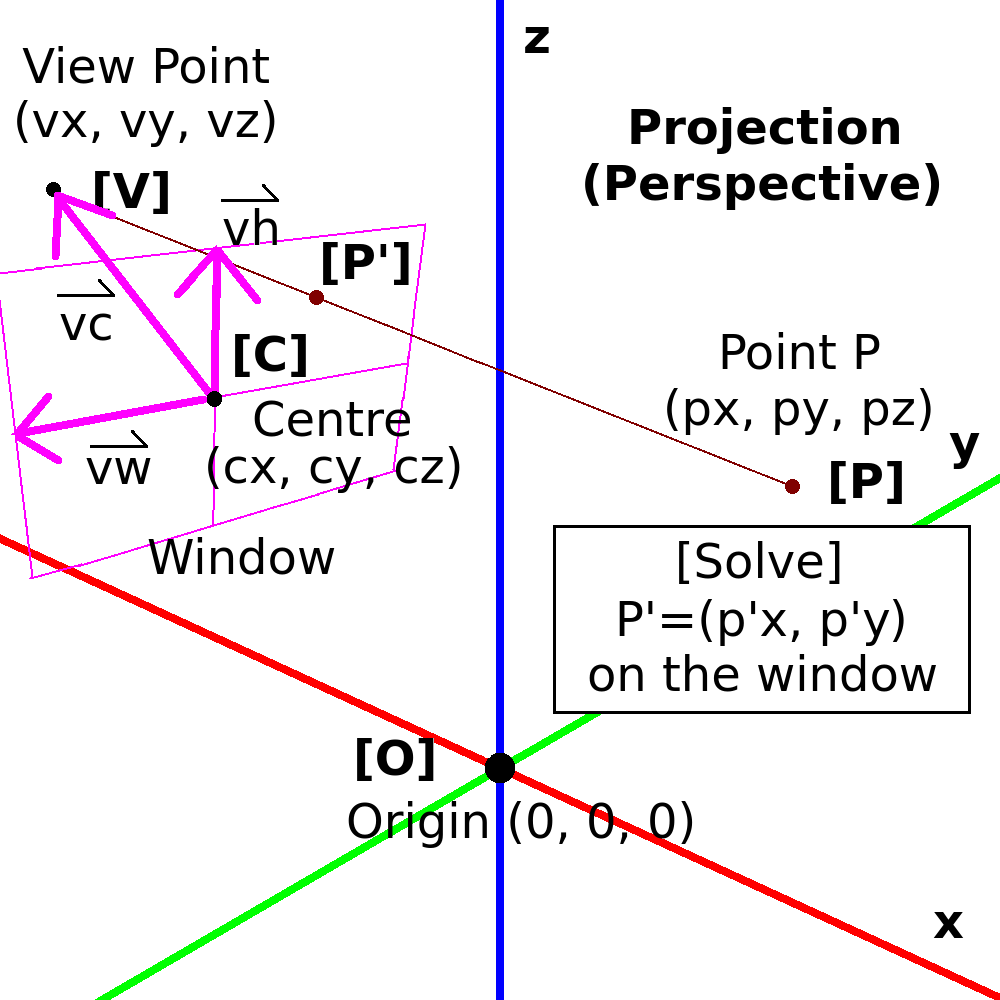
\includegraphics[width=.5\columnwidth]{fig/perspective-projection.png}
		\caption{Projection in Euclidean $\mathbb{R}^3$ Space}
	\end{figure}

\end{frame}


\section{Command}

\subsection{Window}

\subsubsection{Create}

\begin{frame}[t] \frametitle{Create a Window}

	\begin{block}{Command} \newcolumntype{R}{>{\raggedleft\arraybackslash}X}
		\begin{tabularx}{\textwidth}{@{}l@{}l@{}R}
			\InstrName{create window} &
				\ParamMust{\StrName{\ADD\LAB{e}}} & \InstrItem
		\end{tabularx}
	\end{block}

	\begin{block}{Parameters} \begin{itemize}
		\ParamItem{\LAB{e}}   the name of the object from the class window
	\end{itemize} \end{block}

	\begin{block}{Examples}
		\CommandEx{create window main}
	\end{block}

\end{frame}

\subsubsection{Delete}

\begin{frame}[t] \frametitle{Delete a Window}

	\begin{block}{Command} \newcolumntype{R}{>{\raggedleft\arraybackslash}X}
		\begin{tabularx}{\textwidth}{@{}l@{}l@{}l@{}R}
			\InstrName{delete window} &
				\ParamMust{\StrName{\SUB\LAB{e}}} &
			  	\ParamOptl{\StrName{string}} & \InstrItem
		\end{tabularx}
	\end{block}

	\begin{block}{Parameters} \begin{itemize}
		\ParamItem{\LAB{e}}   the name of the object from the class window
		\ParamItem{string}    the text printed right after exiting the current session
	\end{itemize} \end{block}

	\begin{block}{Examples}
		\CommandEx{delete window main}
		\CommandEx{delete window main \QuoteText{Have a nice day.}}
	\end{block}

\end{frame}

\subsubsection{Property}

\begin{frame}[t] \frametitle{Properties of a Window}

	\newcolumntype{R}{>{\raggedright\arraybackslash}X}
	\renewcommand\arraystretch{1.6}
	\begin{tabularx}{\textwidth}{|l|l|R|}
		\hline
		Property         & Value Format & Default \\ \hline
		\hline
		dots-per-cm      & $\Param{\MSR>0}$ & \texttt{128} \\ \hline
		dots-per-unit    & $\Param{\MSR>0}$ & \texttt{256} \\ \hline
		\hline
		background-color & $\Tup{\Param{\MSN\in[0,255]}}{3}$ & \texttt{\TupText{0 0 0}} \\ \hline
	\end{tabularx}

\end{frame}

\subsection{Camera}

\subsubsection{Create}

\begin{frame}[t] \frametitle{Create a Camera}

	\begin{block}{Command} \newcolumntype{R}{>{\raggedleft\arraybackslash}X}
		\begin{tabularx}{\textwidth}{@{}l@{}l@{}l@{}l@{}l@{}R}
			\InstrName{create camera} &
				\ParamMust{\StrName{\ADD\LAB{e}}} &
				\ParamMust{\TupName{\MSR}{3}{center}} &
				\ParamMust{\TupName{\Vct{\MSR}{3}}{2}{plane}} &
				\ParamMust{\VctName{\MSR}{3}{sight}} & \InstrItem
		\end{tabularx}
	\end{block}

	\begin{block}{Parameters} \begin{itemize}
		\ParamItem{\LAB{e}}   the name of the object from the class camera
		\ParamItem{center}    the world coordinate $(c_x, c_y, c_z)$ of the center of the viewport
		\ParamItem{plane}     the horizontal and the vertical vertors $(\vec{v_w}, \vec{v_h})$ of the viewport
		\ParamItem{sight}     the reverse line of sight $\vec{v_c}$ from \Param{center} to the camera
	\end{itemize} \end{block}

	\begin{block}{Examples}
		\CommandEx{create camera z-top \TupText{0 0 1} \TupText{\VctText{2 0 0} \VctText{0 1.5 0}} \VctText{0 0 1}}
		\CommandEx{// The size of the viewport is 512px * 384px when dots-per-unit is 256.}
	\end{block}

\end{frame}

\subsubsection{Select}

\begin{frame}[t] \frametitle{Select a Camera}

	\begin{block}{Command} \newcolumntype{R}{>{\raggedleft\arraybackslash}X}
		\begin{tabularx}{\textwidth}{@{}l@{}l@{}l@{}R}
			\InstrName{select camera} &
				\ParamMust{\StrName{\REF\LABEL{e}{1}}} &
				\ParamMust{\StrName{\REF\LABEL{e}{2}}} & \InstrItem
		\end{tabularx}
	\end{block}

	\begin{block}{Parameters} \begin{itemize}
		\ParamItem{\LABEL{e}{1}} the name of the object from the class camera
		\ParamItem{\LABEL{e}{2}} the name of the object from the class window
	\end{itemize} \end{block}

	\begin{block}{Examples}
		\CommandEx{select camera z-top main}
	\end{block}

\end{frame}

\subsubsection{Remove}

\begin{frame}[t] \frametitle{Remove a Camera}

	\begin{block}{Command} \newcolumntype{R}{>{\raggedleft\arraybackslash}X}
		\begin{tabularx}{\textwidth}{@{}l@{}l@{}l@{}R}
			\InstrName{remove camera} &
				\ParamMust{\StrName{\REF\LABEL{e}{1}}} &
				\ParamMust{\StrName{\REF\LABEL{e}{2}}} & \InstrItem
		\end{tabularx}
	\end{block}

	\begin{block}{Parameters} \begin{itemize}
		\ParamItem{\LABEL{e}{1}} the name of the object from the class camera
		\ParamItem{\LABEL{e}{2}} the name of the object from the class window
	\end{itemize} \end{block}

	\begin{block}{Examples}
		\CommandEx{remove camera z-top main}
	\end{block}

\end{frame}

\subsubsection{Delete}

\begin{frame}[t] \frametitle{Delete a Camera}

	\begin{block}{Command} \newcolumntype{R}{>{\raggedleft\arraybackslash}X}
		\begin{tabularx}{\textwidth}{@{}l@{}l@{}R}
			\InstrName{delete camera} &
				\ParamMust{\StrName{\SUB\LAB{e}}} & \InstrItem
		\end{tabularx}
	\end{block}

	\begin{block}{Parameters} \begin{itemize}
		\ParamItem{\LAB{e}}   the name of the object from the class camera
	\end{itemize} \end{block}

	\begin{block}{Examples}
		\CommandEx{delete camera z-top}
	\end{block}

\end{frame}

\subsubsection{Property}

\begin{frame}[t] \frametitle{Properties of a Camera}

	\newcolumntype{R}{>{\raggedright\arraybackslash}X}
	\renewcommand\arraystretch{1.6}
	\begin{tabularx}{\textwidth}{|l|l|R|}
		\hline
		Property      & Value Format & Default \\ \hline
		\hline
		axis-enable   & $\Param{\MSS\in\{\texttt{true},\texttt{false}\}}$ & \texttt{true} \\ \hline
		axis-show     & $\Param{\MSS\in\{\texttt{x},\texttt{y},\texttt{z},\texttt{xy},\texttt{xz},\texttt{yz},\texttt{xyz}\}}$ & \texttt{xyz} \\ \hline
		axis-color    & $\Tup{\Tup{\Param{\MSN\in[0,255]}}{3}}{3}$ & \texttt{\TupText{\TupText{255 0 0}\TupText{0 255 0}\TupText{0 0 255}}} \\ \hline
		axis-width    & $\LstFull{\Param{\MSR>0} \ \ \Param{\MSS\in\{\texttt{px},\texttt{cm}\}}}$ & \texttt{\LstText{2 px}} \\ \hline
		\hline
		grid-enable   & $\Param{\MSS\in\{\texttt{true},\texttt{false}\}}$ & \texttt{true} \\ \hline
		grid-show     & $\Param{\MSS\in\{\texttt{x},\texttt{y},\texttt{z},\texttt{xy},\texttt{xz},\texttt{yz},\texttt{xyz}\}}$ & \texttt{xy} \\ \hline
		grid-color    & $\Tup{\Tup{\Param{\MSN\in[0,255]}}{3}}{3}$ & \texttt{\TupText{\TupText{127 0 0}\TupText{0 127 0}\TupText{0 0 127}}} \\ \hline
		grid-width    & $\LstFull{\Param{\MSR>0} \ \ \Param{\MSS\in\{\texttt{px},\texttt{cm}\}}}$ & \texttt{\LstText{1 px}} \\ \hline
		grid-interval & $\Param{\MSR>0}$ & \texttt{10} \\ \hline
	\end{tabularx}

\end{frame}

\subsection{Point}

\subsubsection{Create}

\begin{frame}[t] \frametitle{Create Points}

	\begin{block}{Command} \newcolumntype{R}{>{\raggedleft\arraybackslash}X}
		\begin{tabularx}{\textwidth}{@{}l@{}l@{}l@{}R}
			\InstrName{create point } &
			  	\ParamMust{\SetStarOptl{\StrName{\ADD\LAB{p}}}{}} &
			  	\ParamMust{\TupName{\MSR}{3}{coord}} & \InstrItem \\
			\InstrName{create point } &
				\ParamMust{\TupStar{\StrName{\ADD\LAB{p}}}{\,\geqslant n}} &
				\ParamMust{\TupStar{\TupName{\MSR}{3}{coord}}{n}} & \InstrItem
		\end{tabularx}
	\end{block}

	\begin{block}{Parameters} \begin{itemize}
		\ParamItem{\LAB{p}}   the name of the object from the class point
		\ParamItem{coord}     the world coordinate $(p_x, p_y, p_z)$ of the object named \Param{\LAB{p}}
	\end{itemize} \end{block}

	\begin{block}{Examples}
		\CommandEx{create point \QuoteText{origin} \ \ \TupText{0 0 0}}
		\CommandEx{create point \SetText{X-1 X-2} \ \TupText{1 0 0}}
		\CommandEx{create point \TupText{Y-1 Y-2} \TupText{\TupText{0 1 0}}}
		\CommandEx{create point \TupText{Z D1 D2} \TupText{\TupText{0 1 0} \TupText{1 1 1}}}
	\end{block}

\end{frame}

\subsubsection{Delete}

\begin{frame}[t] \frametitle{Delete Points}

	\begin{block}{Command} \newcolumntype{R}{>{\raggedleft\arraybackslash}X}
		\begin{tabularx}{\textwidth}{@{}l@{}l@{}R}
			\InstrName{delete point } &
				\ParamMust{\SetStarOptl{\StrName{\SUB\LAB{p}}}{}} & \InstrItem
		\end{tabularx}
	\end{block}

	\begin{block}{Parameters} \begin{itemize}
		\ParamItem{\LAB{p}}   the name of the object from the class point
	\end{itemize} \end{block}

	\begin{block}{Examples}
		\CommandEx{delete point \QuoteText{origin}}
		\CommandEx{delete point \SetText{Z D1 D2}}
	\end{block}

\end{frame}

\subsubsection{Property}

\begin{frame}[t] \frametitle{Properties of a Point}

	\newcolumntype{R}{>{\raggedright\arraybackslash}X}
	\renewcommand\arraystretch{1.6}
	\begin{tabularx}{\textwidth}{|l|l|R|}
		\hline
		Property     & Value Format & Default \\ \hline
		\hline
		shape        & $\Param{\MSS\in\{\texttt{none},\texttt{dot},\texttt{square}\}}$ & \texttt{dot} \\ \hline
		radius       & $\LstFull{\Param{\MSR>0} \ \ \Param{\MSS\in\{\texttt{px},\texttt{cm}\}}}$ & \texttt{\LstText{3 px}} \\ \hline
        color        & $\Tup{\Param{\MSN\in[0,255]}}{3}$ & \texttt{\TupText{255 255 255}} \\ \hline
        \hline
		border-type  & $\Param{\MSS\in\{\texttt{none},\texttt{inner},\texttt{middle},\texttt{outer}\}}$ & \texttt{outer} \\ \hline
		border-width & $\LstFull{\Param{\MSR>0} \ \ \Param{\MSS\in\{\texttt{px},\texttt{cm}\}}}$ & \texttt{\LstText{2 px}} \\ \hline
        border-color & $\Tup{\Param{\MSN\in[0,255]}}{3}$ & \texttt{\TupText{127 127 127}} \\ \hline
	\end{tabularx}

\end{frame}

\subsection{Line}

\subsubsection{Create}

\begin{frame}[t] \frametitle{Create Line Segments}

	\begin{block}{Command} \newcolumntype{R}{>{\raggedleft\arraybackslash}X}
		\begin{tabularx}{\textwidth}{@{}l@{}l@{}l@{}R}
			\InstrName{create line \ } &
			  	\ParamMust{\SetStarOptl{\StrName{\ADD\LAB{c}}}{}} &
			  	\ParamMust{\Set{\StrName{\REF\LAB{p}}}{2}} & \InstrItem \\
			\InstrName{create line \ } &
				\ParamMust{\TupStar{\StrName{\ADD\LAB{c}}}{\,\geqslant n}} &
				\ParamMust{\TupStar{\Set{\StrName{\REF\LAB{p}}}{2}}{n}} & \InstrItem
		\end{tabularx}
	\end{block}

	\begin{block}{Parameters} \begin{itemize}
		\ParamItem{\LAB{c}}   the name of the object from the class line
		\ParamItem{\LAB{p}}   the name of the object from the class point
	\end{itemize} \end{block}

	\begin{block}{Examples}
		\CommandEx{create line \ seg-1 \quad \quad \quad \ \SetText{X-1 Y-1}}
		\CommandEx{create line \SetText{seg-2 seg-3} \SetText{X-2 Y-2}}
	\end{block}

\end{frame}

\subsubsection{Delete}

\begin{frame}[t] \frametitle{Delete Line Segments}

	\begin{block}{Command} \newcolumntype{R}{>{\raggedleft\arraybackslash}X}
		\begin{tabularx}{\textwidth}{@{}l@{}l@{}R}
			\InstrName{delete line \ } &
			  	\ParamMust{\SetStarOptl{\StrName{\SUB\LAB{c}}}{}} & \InstrItem
		\end{tabularx}
	\end{block}

	\begin{block}{Parameters} \begin{itemize}
		\ParamItem{\LAB{c}}   the name of the object from the class line
	\end{itemize} \end{block}

	\begin{block}{Examples}
		\CommandEx{delete line \ seg-1}
		\CommandEx{delete line \SetText{seg-2 seg-3}}
	\end{block}

\end{frame}

\subsubsection{Property}

\begin{frame}[t] \frametitle{Properties of a Line}

	\newcolumntype{R}{>{\raggedright\arraybackslash}X}
	\renewcommand\arraystretch{1.6}
	\begin{tabularx}{\textwidth}{|l|l|R|}
		\hline
		Property & Value Format & Default \\ \hline
		\hline
		style    & $\Param{\MSS\in\{\texttt{none},\texttt{solid},\texttt{dotted},\texttt{dashed}\}}$ & \texttt{solid} \\ \hline
		width    & $\LstFull{\Param{\MSR>0} \ \ \Param{\MSS\in\{\texttt{px},\texttt{cm}\}}}$ & \texttt{\LstText{2 px}} \\ \hline
        color    & $\Tup{\Param{\MSN\in[0,255]}}{3}$ & \texttt{\TupText{191 191 191}} \\ \hline
        \hline
        cap      & $\MSS\in\{\texttt{butt},\texttt{round},\texttt{square}\}$ & \texttt{butt} \\ \hline
        pattern  & $\LstFull{\Tup{\Param{\MSR>0}}{} \ \Param{\MSS\in\{\texttt{px},\texttt{cm}\}}}$ & \texttt{\LstText{\TupText{8 8} px}} \\ \hline
	\end{tabularx}

\end{frame}

\subsection{Attribute}

\subsubsection{Create}

\begin{frame}[t] \frametitle{Create Attributes}

	\begin{block}{Command} \newcolumntype{R}{>{\raggedleft\arraybackslash}X}
		\begin{tabularx}{\textwidth}{@{}l@{}l@{}l@{}R}
			\InstrName{create attrib} &
				\ParamMust{\SetStarOptl{\StrName{\ADD\LAB{a}}}{}} &
				\ParamMust{\LstStarOptl{\LstFull{\StrName{\CLS{pc}} \ \LstOptl{\StrName{prop} \ \StrName{value}}{}}}{}} & \InstrItem \\
			\InstrName{create attrib} &
				\ParamMust{\TupStar{\StrName{\ADD\LAB{a}}}{}} &
				\ParamMust{\LstStar{\LstFull{\StrName{\CLS{pc}} \ \LstOptl{\StrName{prop} \ \StrName{value}}{}}}{}} & \InstrItem
		\end{tabularx}
	\end{block}

	\begin{block}{Parameters} \begin{itemize}
		\ParamItem{\LAB{a}}   the name of the object from the class attrib
		\ParamItem{\CLS{pc}}  the name of a class in the field primitive or compound
		\ParamItem{prop}      the property of the object from \Param{\CLS{pc}}
		\ParamItem{value}     the value of \Param{prop} in the designated format
	\end{itemize} \end{block}

	\begin{block}{Examples}
		\CommandEx{create attrib \TupText{purple dashed-and-translucent-line} \EOLText
		                         \LstText{\LstText{point color \QuoteText{\TupText{128 0 128}}} \EOLText
		                       \ \LstText{line \LstText{style dashed} \LstText{color \QuoteText{\TupText{0 255 0}}} \LstText{pattern \QuoteText{\LstText{\TupText{16 8} px}}}}}}
	\end{block}

\end{frame}

\subsubsection{Attach}

\begin{frame}[t] \frametitle{Attach Attributes}

	\begin{block}{Command} \newcolumntype{R}{>{\raggedleft\arraybackslash}X}
		\begin{tabularx}{\textwidth}{@{}l@{}l@{}l@{}R}
			\InstrName{attach attrib} &
				\ParamMust{\TupStarOptl{\StrName{\REF\LAB{a}}}{}} &
				\ParamMust{\SetStarOptl{\StrName{\REF\LAB{pc}}}{}} & \InstrItem \\
			\InstrName{attach attrib} &
				\ParamMust{\TupStar{\StrName{\REF\LAB{a}}}{}} &
				\ParamMust{\TupStar{\StrName{\REF\LAB{pc}}}{}} & \InstrItem
		\end{tabularx}
	\end{block}

	\begin{block}{Parameters} \begin{itemize}
		\ParamItem{\LAB{a}}   the name of the object from the class attrib
		\ParamItem{\LAB{pc}}  the name of the object from a class in the field primitive or compound
	\end{itemize} \end{block}

	\begin{block}{Examples}
		\CommandEx{attach attrib \ red \quad \quad \quad \ \ point-0}
		\CommandEx{attach attrib \TupText{red large} \ point-1}
		\CommandEx{attach attrib \ blue \quad \quad \quad \SetText{point-2 rect-0}}
		\CommandEx{attach attrib \TupText{5px black} \SetText{point-3 circ-0}}
		\CommandEx{attach attrib \TupText{red thick} \TupText{point-4 line-0 triangle-0}}
	\end{block}

\end{frame}

\subsubsection{Detach}

\begin{frame}[t] \frametitle{Detach Attributes}

	\begin{block}{Command} \newcolumntype{R}{>{\raggedleft\arraybackslash}X}
		\begin{tabularx}{\textwidth}{@{}l@{}l@{}l@{}R}
			\InstrName{detach attrib} &
				\ParamMust{\SetStarOptl{\StrName{\REF\LAB{a}}}{}} &
				\ParamMust{\SetStarOptl{\StrName{\REF\LAB{pc}}}{}} & \InstrItem \\
			\InstrName{detach attrib} &
				\ParamMust{\TupStar{\StrName{\REF\LAB{a}}}{}} &
				\ParamMust{\TupStar{\StrName{\REF\LAB{pc}}}{}} & \InstrItem
		\end{tabularx}
	\end{block}

	\begin{block}{Parameters} \begin{itemize}
		\ParamItem{\LAB{a}}   the name of the object from the class attrib
		\ParamItem{\LAB{pc}}  the name of the object from a class in the field primitive or compound
	\end{itemize} \end{block}

	\begin{block}{Examples}
		\CommandEx{detach attrib \ red \quad \quad \quad \ \ point-0}
		\CommandEx{detach attrib \SetText{red large} \ point-1}
		\CommandEx{detach attrib \ blue \quad \quad \quad \SetText{point-2 rect-0}}
		\CommandEx{detach attrib \SetText{5px black} \SetText{point-3 circ-0}}
		\CommandEx{detach attrib \TupText{red thick} \TupText{point-4 line-0 triangle-0}}
	\end{block}

\end{frame}

\subsubsection{Delete}

\begin{frame}[t] \frametitle{Delete Attributes}

	\begin{block}{Command} \newcolumntype{R}{>{\raggedleft\arraybackslash}X}
		\begin{tabularx}{\textwidth}{@{}l@{}l@{}R}
			\InstrName{delete attrib} &
				\ParamMust{\SetStarOptl{\StrName{\SUB\LAB{a}}}{}} & \InstrItem
		\end{tabularx}
	\end{block}

	\begin{block}{Parameters} \begin{itemize}
		\ParamItem{\LAB{a}}   the name of the object from the class attrib
	\end{itemize} \end{block}

	\begin{block}{Examples}
		\CommandEx{delete attrib \ red}
		\CommandEx{delete attrib \SetText{5px large}}
	\end{block}

\end{frame}

\subsection{Operation}

\subsubsection{Assign}

\begin{frame}[t] \frametitle{Assign Operations}

	\begin{block}{Command} \newcolumntype{R}{>{\raggedleft\arraybackslash}X}
		\begin{tabularx}{\textwidth}{@{}l@{}l@{}l@{}l@{}R}
			\InstrName{assign operat} &
				\ParamMust{\StrName{action}} &
				\ParamMust{\StrName{class}} &
				\ParamOptl{\MSNName{repeat}\ \ValueDefn{=\infty}} & \InstrItem
		\end{tabularx}
	\end{block}

	\begin{block}{Parameters} \begin{itemize}
		\ParamItem{action}    the name of the corresponding action of \Param{class}
		\ParamItem{class}     the name of a class
		\ParamItem{repeat}    the amount of the commands emitting operation names
	\end{itemize} \end{block}

	\begin{block}{Examples}
		\CommandEx{assign operat create point 2}
		\CommandEx{x-axis \TupText{1 0 0}}
		\CommandEx{y-axis \TupText{0 1 0}}
		\CommandEx{// Back To Normal}
	\end{block}

\end{frame}


\end{document}

